\documentclass{article}

\usepackage{amsmath}
\usepackage{listings}
\usepackage{graphicx}
\usepackage{xcolor}
\usepackage[parfill]{parskip}

\definecolor{codegreen}{rgb}{0,0.6,0}
\definecolor{codegray}{rgb}{0.5,0.5,0.5}
\definecolor{codepurple}{rgb}{0.58,0,0.82}
\definecolor{backcolour}{rgb}{0.95,0.95,0.92}

\lstdefinestyle{mystyle}{
    backgroundcolor=\color{backcolour},   
    commentstyle=\color{codegreen},
    keywordstyle=\color{magenta},
    numberstyle=\tiny\color{codegray},
    stringstyle=\color{codepurple},
    basicstyle=\ttfamily\footnotesize,
    breakatwhitespace=false,         
    breaklines=true,                 
    captionpos=b,                    
    keepspaces=true,                 
    numbers=left,                    
    numbersep=5pt,                  
    showspaces=false,                
    showstringspaces=false,
    showtabs=false,                  
    tabsize=2
}

\lstset{style=mystyle}

\begin{document}

\begin{titlepage}
\begin{center}
\vspace*{1cm}
		
\textbf{Lab 5}
			
\vspace{0.5cm}
Chengxuan Li
			
\vspace{0.1cm}
1631060
			
\vspace{0.1cm}
Section 801
			
\vspace{0.1cm}
Nov 22nd, 2021
\end{center}
\end{titlepage}

\section*{Question 1}

(b) Sampling rate is 22050 Hz. The bit-rate is 176400 kbps. The duration is 18.1406 seconds.
\begin{lstlisting}[language=Matlab]
[x, Fs] = audioread("love_mono22.wav");
bit = 8;
bitRate = Fs * bit;
duration = length(x) / Fs;
\end{lstlisting}

\section*{Question 2}

(a) Code to calculate DFT
\begin{lstlisting}[language=Matlab]
[x, Fs] = audioread("love_mono22.wav");
X = fft(x);
\end{lstlisting}

(b) $X[0]=-16.0625$, $X[1]=0.7786-0.6406i$, $X[2]=3.1697-1.6708i$

(c) Code for scaling $X[r]$
\begin{lstlisting}[language=Matlab]
[x, Fs] = audioread("love_mono22.wav");

X = fft(x); % DFT of the audio signal

N = length(x);
scaledX = X / sqrt(N); % scaled X[r], X'[r]
\end{lstlisting}

(d) Code to generate magnitude plot (in dB) and scaling of frequency axis
\begin{lstlisting}[language=Matlab]
[x, Fs] = audioread("love_mono22.wav");

X = fft(x); % DFT of the audio signal

N = length(x);
scaledX = X / sqrt(N); % scaled X[r], X'[r]

magScaledX = abs(scaledX); % Absolute value of X'[r]

fm = Fs / N / 1000 * (0:N/2);
dbScaledX = 20 * log10(magScaledX(1:N / 2 + 1));

plot(fm, dbScaledX);
title("Magnitude Spectrum Plot of x[k]");
xlabel("Frequency (KHz)");
ylabel("Magnitude of X'[r] (dB)");
\end{lstlisting}

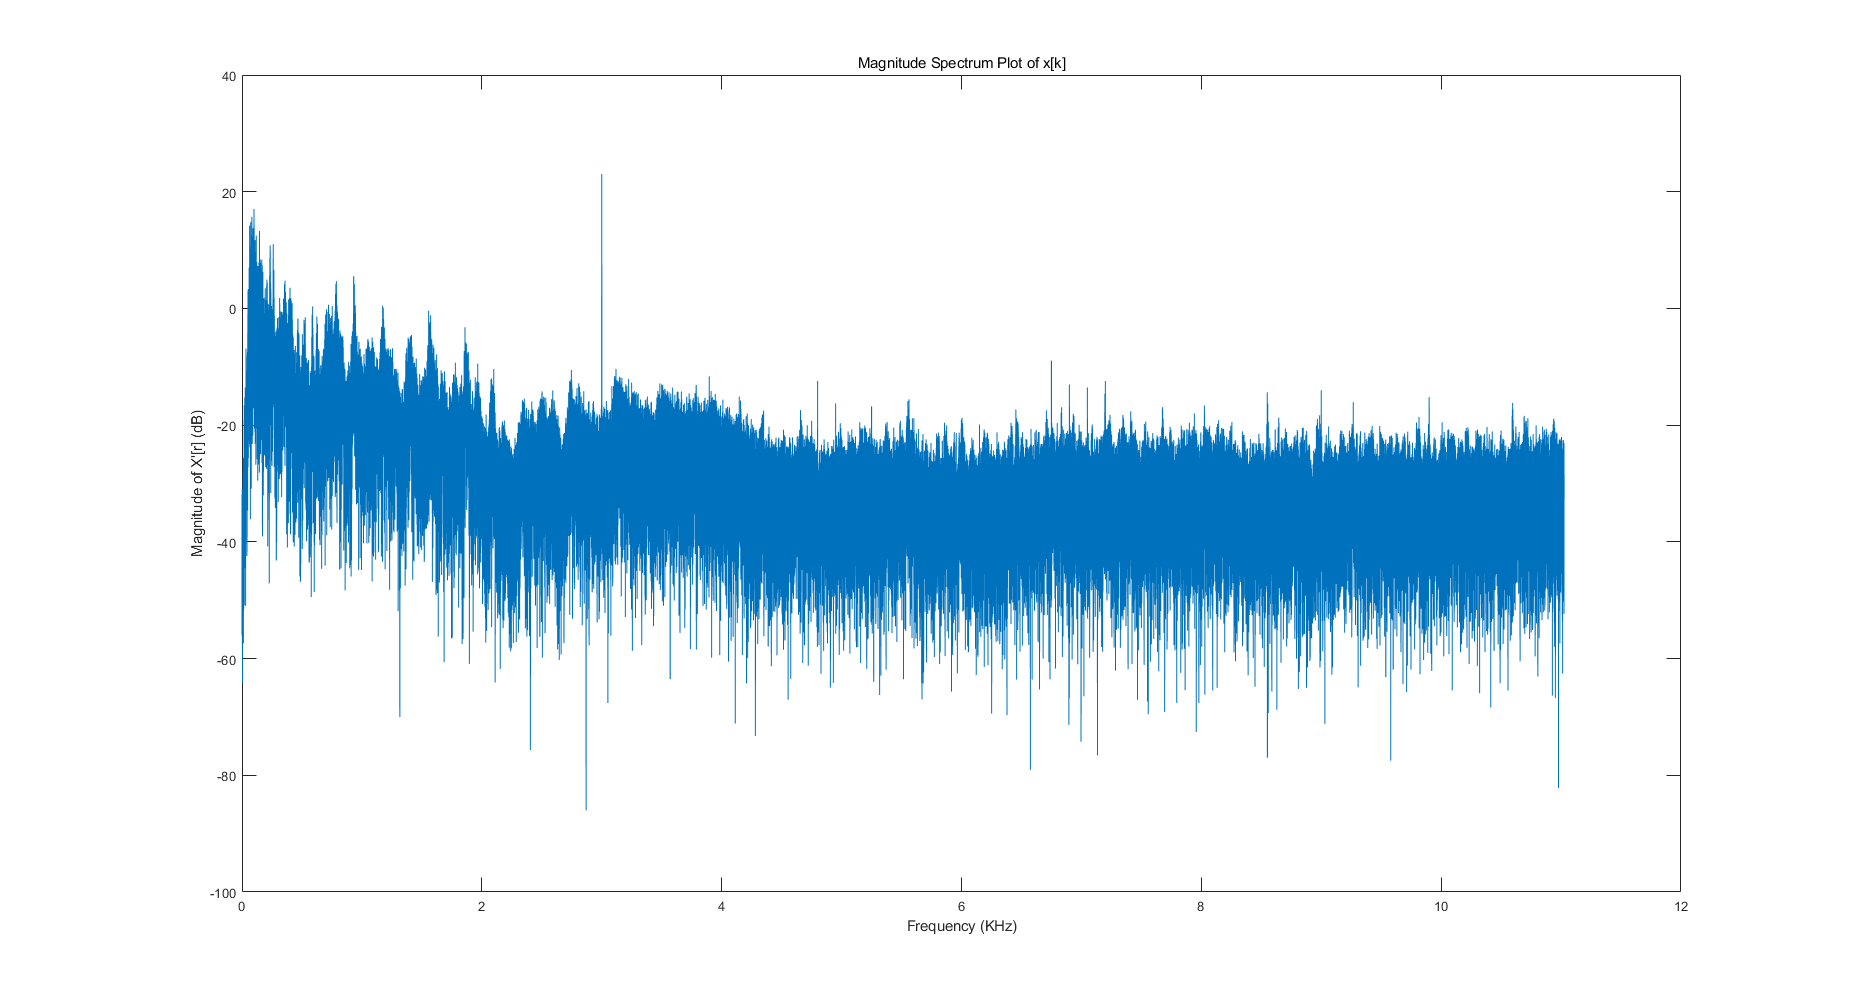
\includegraphics[width=\textwidth]{q2.png}

(e) The frequency intervals corresponding to the m-th coefficient with positive magnitude in dB are around 0 Hz to 400 Hz, 800 Hz and 1 KHz. Those frequency range corresponds to main components of the music such as human voice, instrument and etc. Region around 3 KHz has a significant jump on the positive magnitude axis compared to the magnitude of nearby frequency region. This indicate that the frequency of the noise / distortion is around 3 KHz.

\section*{Question 3}

(a) Generated pwelch plot

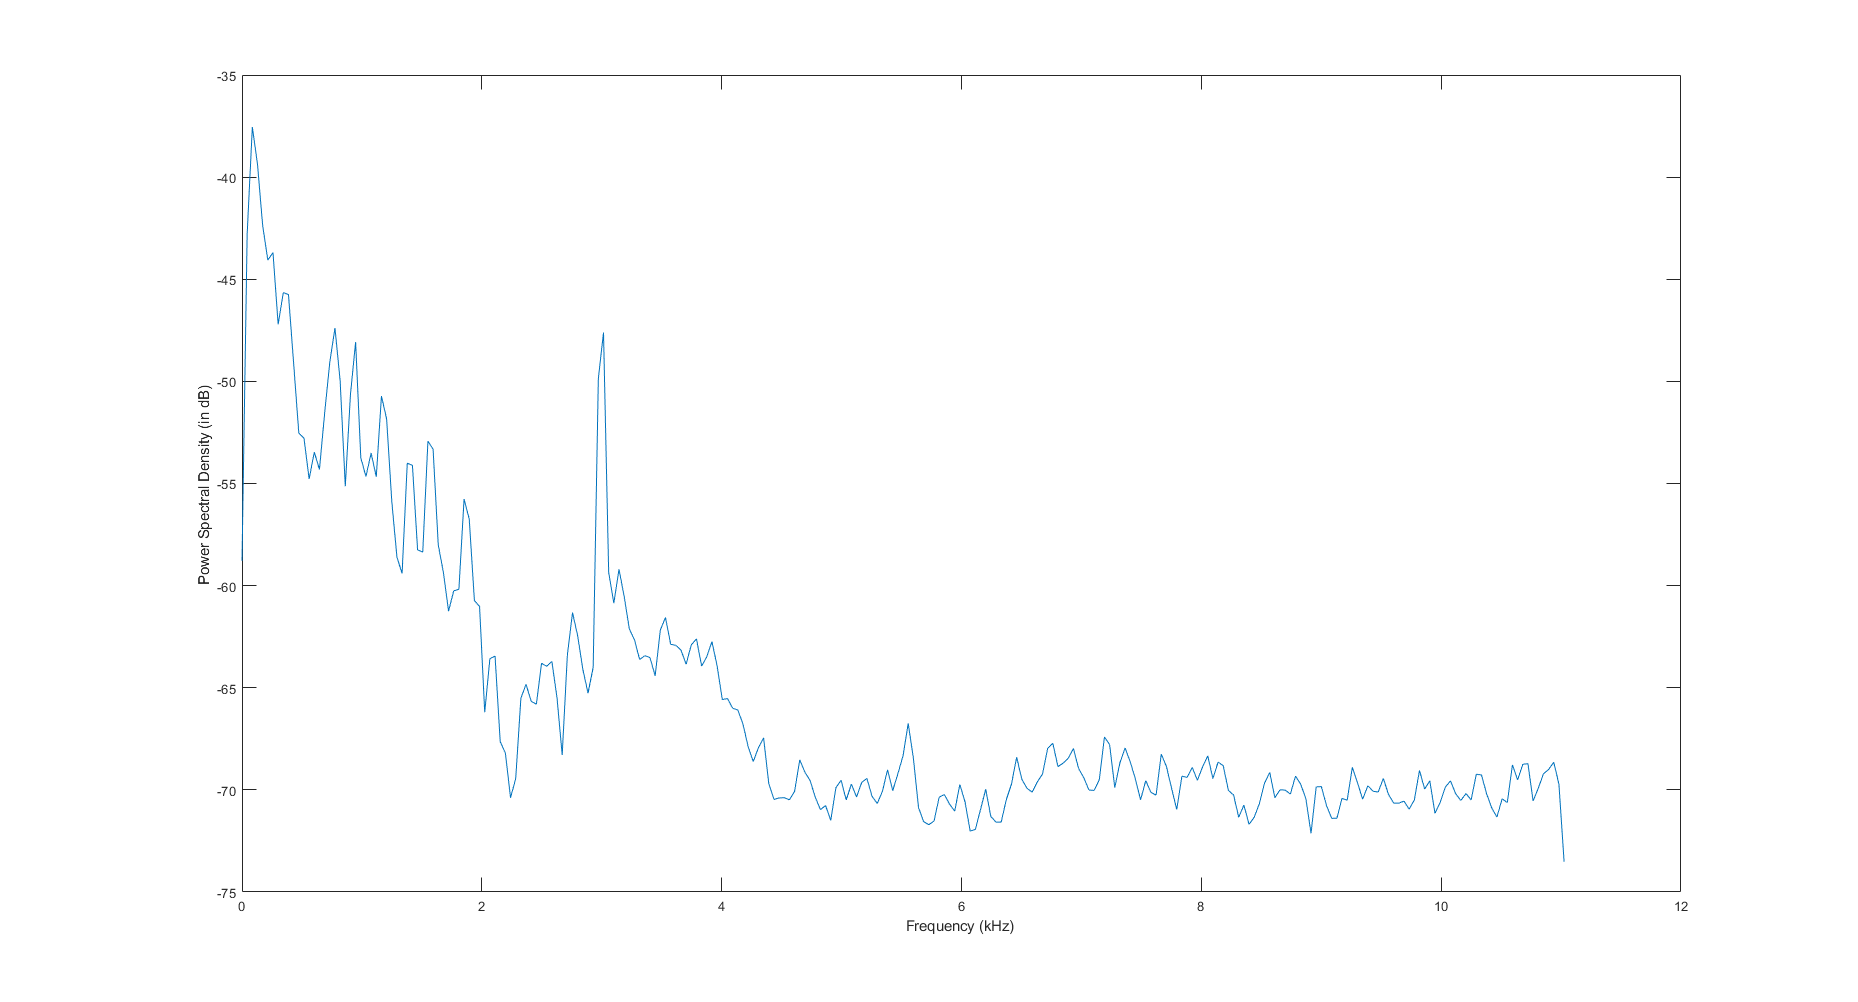
\includegraphics[width=\textwidth]{q3.png}

(b) The frequency range from 0 KHz to 1.7 (1.8) KHz has most energy. Also, the frequency region of 3 KHz also has the similar energy compared to frequency range from 0 KHz to 2KHz.

(c) The frequency of the tonal noise present in the signal is 3 KHz.

\section*{Question 4}

(b) There are annoying artifacts located at the location that have relative complex shapes such as the ears, the white dots scatter in the hair and so on.

(c) Generated Spectrum of the image

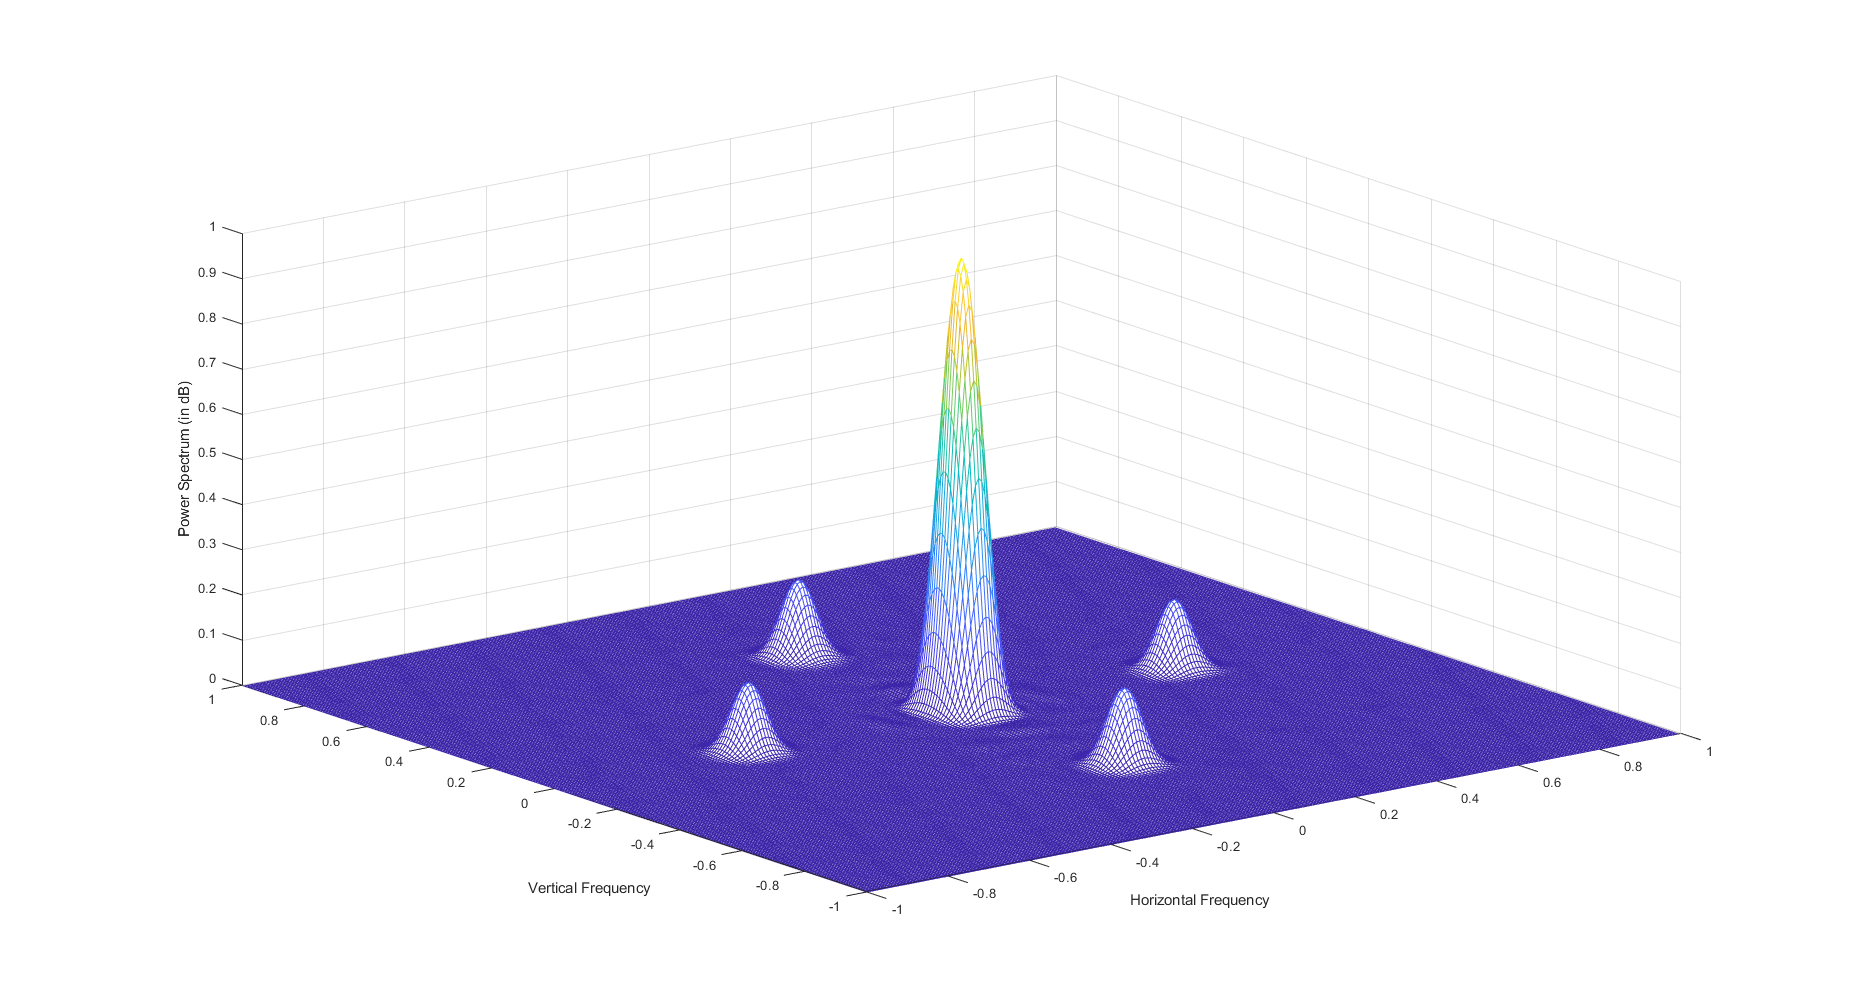
\includegraphics[width=\textwidth]{q4.png}

(d) 2-D frequencies of the noise peaks: (0, 0.523438), (-0.523438, 0), (0, -0.523438), (0.523438, 0).

\end{document}